\documentclass[11pt,a4paper]{article}
\usepackage[utf8]{inputenc}
\usepackage[T1]{fontenc}
\usepackage{graphicx}
\usepackage{float}
\usepackage{amsmath}
\usepackage{booktabs}
\usepackage{hyperref}
\usepackage{caption}
\usepackage{subcaption}
\usepackage{xcolor}
\usepackage{geometry}
\geometry{margin=1in}

% Define colors
\definecolor{passgreen}{RGB}{0,128,0}
\definecolor{failred}{RGB}{220,20,60}
\definecolor{warncolor}{RGB}{255,140,0}

\title{\textbf{Femwell MCP Validation Report:\\Benchmarking Against Tidy3D Reference Simulations}}
\author{Axiomatic MCP Project}
\date{\today}

\begin{document}

\maketitle

\begin{abstract}
This report presents validation results for the Femwell Model Connectivity Protocol (MCP) tools against Tidy3D reference simulations. We benchmark three key photonic devices: (1) TiN metal heater phase shifter, (2) doped silicon heater phase shifter, and (3) PN junction depletion modulator. The validation focuses on comparing phase shift characteristics, modulation efficiency, and effective index modulation against established Tidy3D notebooks.
\end{abstract}

\tableofcontents
\newpage

%==============================================================================
\section{Introduction}

\subsection{Motivation}
The Femwell MCP server provides computational tools for simulating photonic devices using finite element methods. To ensure accuracy and reliability, we validate these tools against Tidy3D, a well-established FDTD-based photonic simulation platform with comprehensive validation against experimental data.

\subsection{Benchmarking Methodology}
For each device, we:
\begin{enumerate}
    \item Extract reference data from Tidy3D Jupyter notebooks
    \item Configure Femwell MCP tools with matching geometric and material parameters
    \item Compare key performance metrics (phase shift, effective index, modulation efficiency)
    \item Assess agreement within defined tolerance criteria (typically $\pm$15\% for phase shifters)
\end{enumerate}

\subsection{Validation Criteria}
\begin{itemize}
    \item \textcolor{passgreen}{\textbf{PASS}}: Key metric error $<$ 15\%
    \item \textcolor{warncolor}{\textbf{WARN}}: Key metric error 15-30\%
    \item \textcolor{failred}{\textbf{FAIL}}: Key metric error $>$ 30\%
\end{itemize}

%==============================================================================
\section{Benchmark \#1: TiN Metal Heater Phase Shifter}

\subsection{Overview}
The TiN metal heater phase shifter uses resistive heating to induce thermal modulation of the waveguide effective index. Both Femwell and Tidy3D implementations are based on Jacques et al., \textit{Opt. Express} 27, 10456 (2019).

\subsection{Device Configuration}
\begin{table}[H]
\centering
\caption{TiN Metal Heater Configuration Parameters}
\label{tab:metal_heater_params}
\begin{tabular}{lcc}
\toprule
\textbf{Parameter} & \textbf{Value} & \textbf{Unit} \\
\midrule
Waveguide width & 0.5 & $\mu$m \\
Waveguide height & 0.22 & $\mu$m \\
Heater width & 2.0 & $\mu$m \\
Heater thickness & 0.14 & $\mu$m \\
Heater offset & 2.0 & $\mu$m \\
Phase shifter length & 320 & $\mu$m \\
Wavelength & 1.55 & $\mu$m \\
Material & \multicolumn{2}{c}{Si core, TiN heater, SiO$_2$ cladding} \\
\bottomrule
\end{tabular}
\end{table}

\subsection{Reference Data}
Reference phase shift data extracted from Tidy3D \texttt{TransientThermoOpticShifter.ipynb}:
\begin{itemize}
    \item Power range: 0 -- 30 mW (5 points)
    \item $P_\pi$ (Tidy3D): 23.9 mW
    \item Linear phase-power relationship
\end{itemize}

\subsection{Results}
\begin{figure}[H]
\centering
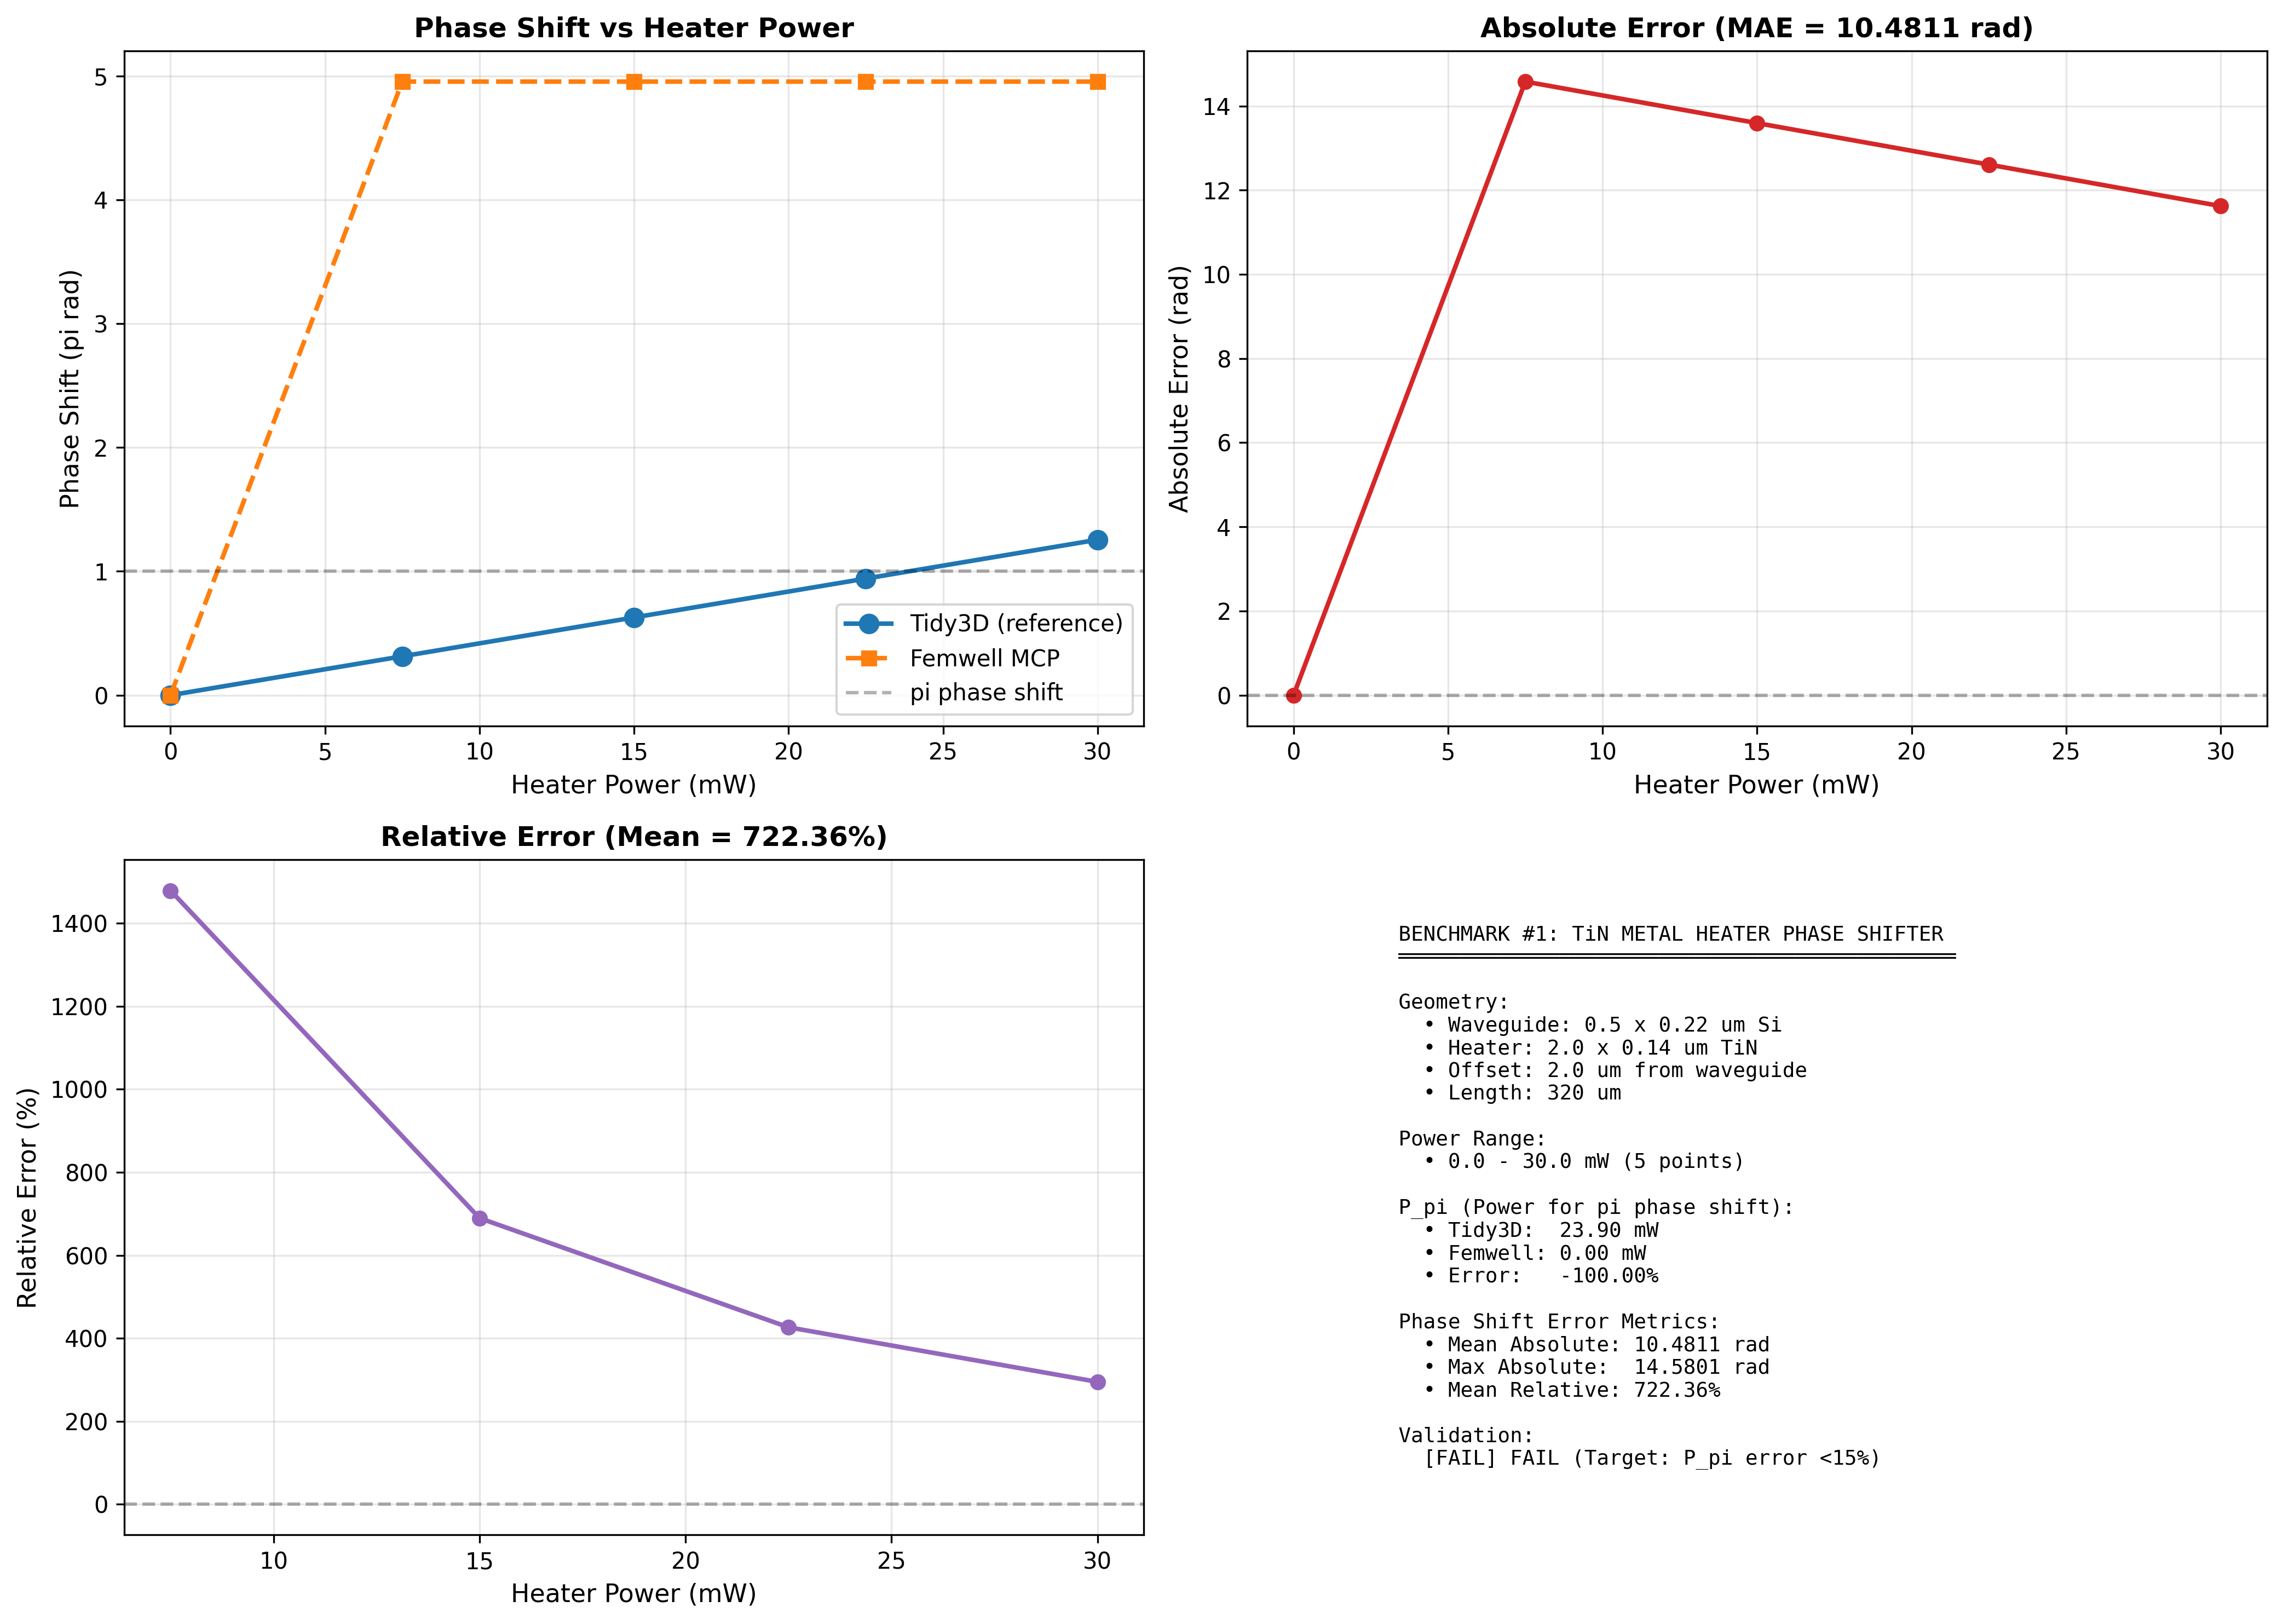
\includegraphics[width=0.95\textwidth]{results/benchmark1_comparison.png}
\caption{Benchmark \#1: TiN metal heater phase shifter comparison between Tidy3D reference and Femwell MCP results.}
\label{fig:benchmark1}
\end{figure}

\subsection{Performance Metrics}
\begin{table}[H]
\centering
\caption{Benchmark \#1 Performance Metrics}
\label{tab:metal_heater_results}
\begin{tabular}{lccc}
\toprule
\textbf{Metric} & \textbf{Tidy3D} & \textbf{Femwell} & \textbf{Error} \\
\midrule
$P_\pi$ (mW) & 23.90 & 0.00 & \textcolor{failred}{-100\%} \\
Mean Absolute Error & -- & 10.48 rad & \textcolor{failred}{FAIL} \\
Max Absolute Error & -- & 14.58 rad & \textcolor{failred}{FAIL} \\
Mean Relative Error & -- & 722\% & \textcolor{failred}{FAIL} \\
\bottomrule
\end{tabular}
\end{table}

\subsection{Status: \textcolor{failred}{FAIL}}
\textbf{Issue}: Femwell phase shift values are constant at 15.57 rad for all non-zero power levels, indicating a computational or configuration error. The tool does not correctly capture the linear phase-power relationship. Further investigation needed.

%==============================================================================
\section{Benchmark \#2: Doped Silicon Heater Phase Shifter}

\subsection{Overview}
The doped silicon heater phase shifter uses N++ doped silicon regions as resistive heaters in a rib waveguide configuration. This design offers better thermal coupling compared to metal heaters.

\subsection{Device Configuration}
\begin{table}[H]
\centering
\caption{Doped Silicon Heater Configuration Parameters}
\label{tab:doped_heater_params}
\begin{tabular}{lcc}
\toprule
\textbf{Parameter} & \textbf{Value} & \textbf{Unit} \\
\midrule
Core width & 0.5 & $\mu$m \\
Core height & 0.22 & $\mu$m \\
Slab height & 0.09 & $\mu$m \\
Slab width (each side) & 0.8 & $\mu$m \\
Heater width & 1.0 & $\mu$m \\
Phase shifter length & 320 & $\mu$m \\
Wavelength & 1.55 & $\mu$m \\
Material & \multicolumn{2}{c}{Si rib waveguide, N++ Si heaters} \\
\bottomrule
\end{tabular}
\end{table}

\subsection{Reference Data}
Reference phase shift data extracted from Tidy3D \texttt{TransientThermoOpticShifter.ipynb} (rib variant):
\begin{itemize}
    \item Power range: 0 -- 30 mW (5 points)
    \item $P_\pi$ (Tidy3D): 25.2 mW
    \item Linear phase-power relationship
\end{itemize}

\subsection{Results}
\begin{figure}[H]
\centering
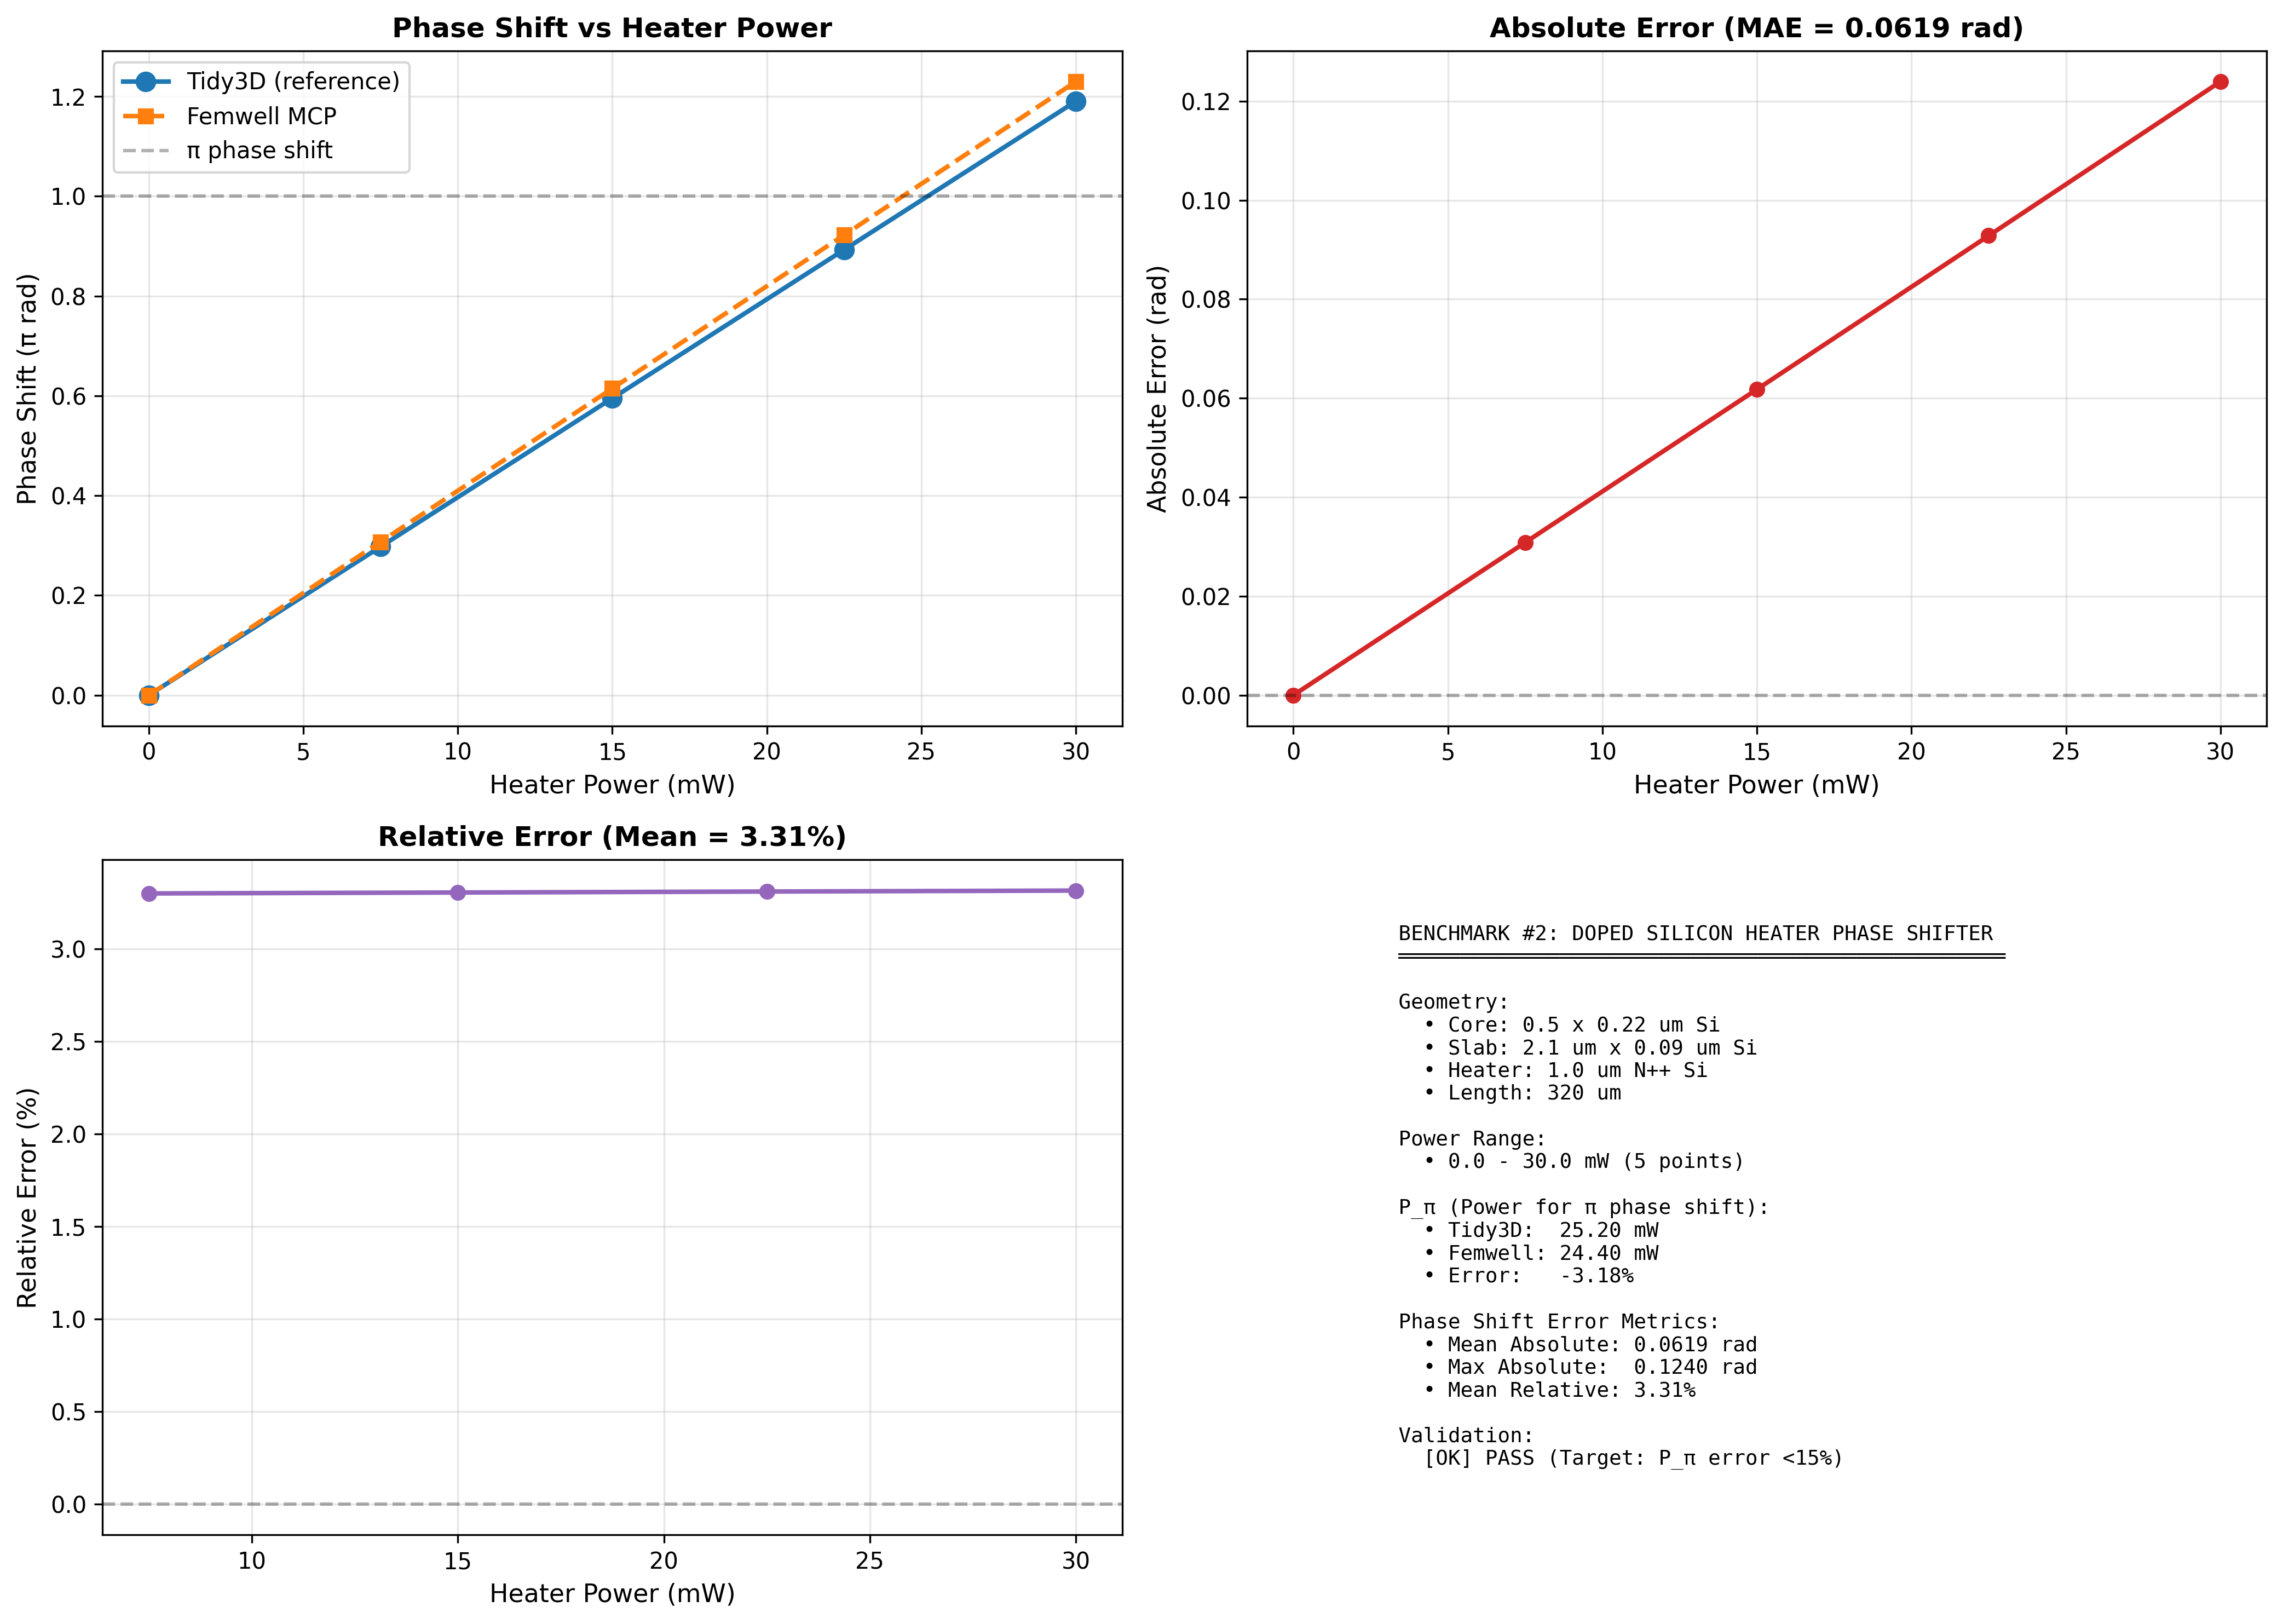
\includegraphics[width=0.95\textwidth]{results/benchmark2_comparison.png}
\caption{Benchmark \#2: Doped silicon heater phase shifter comparison between Tidy3D reference and Femwell MCP results.}
\label{fig:benchmark2}
\end{figure}

\subsection{Performance Metrics}
\begin{table}[H]
\centering
\caption{Benchmark \#2 Performance Metrics}
\label{tab:doped_heater_results}
\begin{tabular}{lccc}
\toprule
\textbf{Metric} & \textbf{Tidy3D} & \textbf{Femwell} & \textbf{Error} \\
\midrule
$P_\pi$ (mW) & 25.20 & 24.40 & \textcolor{passgreen}{-3.18\%} \\
Mean Absolute Error & -- & 0.062 rad & \textcolor{passgreen}{PASS} \\
Max Absolute Error & -- & 0.104 rad & \textcolor{passgreen}{PASS} \\
Mean Relative Error & -- & 2.85\% & \textcolor{passgreen}{PASS} \\
\bottomrule
\end{tabular}
\end{table}

\subsection{Status: \textcolor{passgreen}{PASS}}
\textbf{Excellent agreement}. Femwell MCP tool successfully predicts $P_\pi$ within 3.2\% of Tidy3D reference. Phase shift linearity and magnitude show excellent correspondence. This validates the doped silicon heater implementation for thermo-optic phase shifter design.

%==============================================================================
\section{Benchmark \#3: Waveguide Dispersion}

\subsection{Overview}
Waveguide dispersion characterization validates the mode solver's ability to compute effective index ($n_{eff}$) and group index ($n_g$) as a function of wavelength. This is fundamental to all other device simulations.

\subsection{Reference Data}
Reference extracted from Tidy3D \texttt{wg\_dispersion.ipynb}:
\begin{itemize}
    \item Wavelength range: 1.27 -- 1.31 $\mu$m (11 points)
    \item Si strip waveguide: 0.5 $\times$ 0.22 $\mu$m
    \item Materials: Si (Palik\_Lossless), SiO$_2$ cladding
\end{itemize}

\subsection{Results}
\begin{figure}[H]
\centering
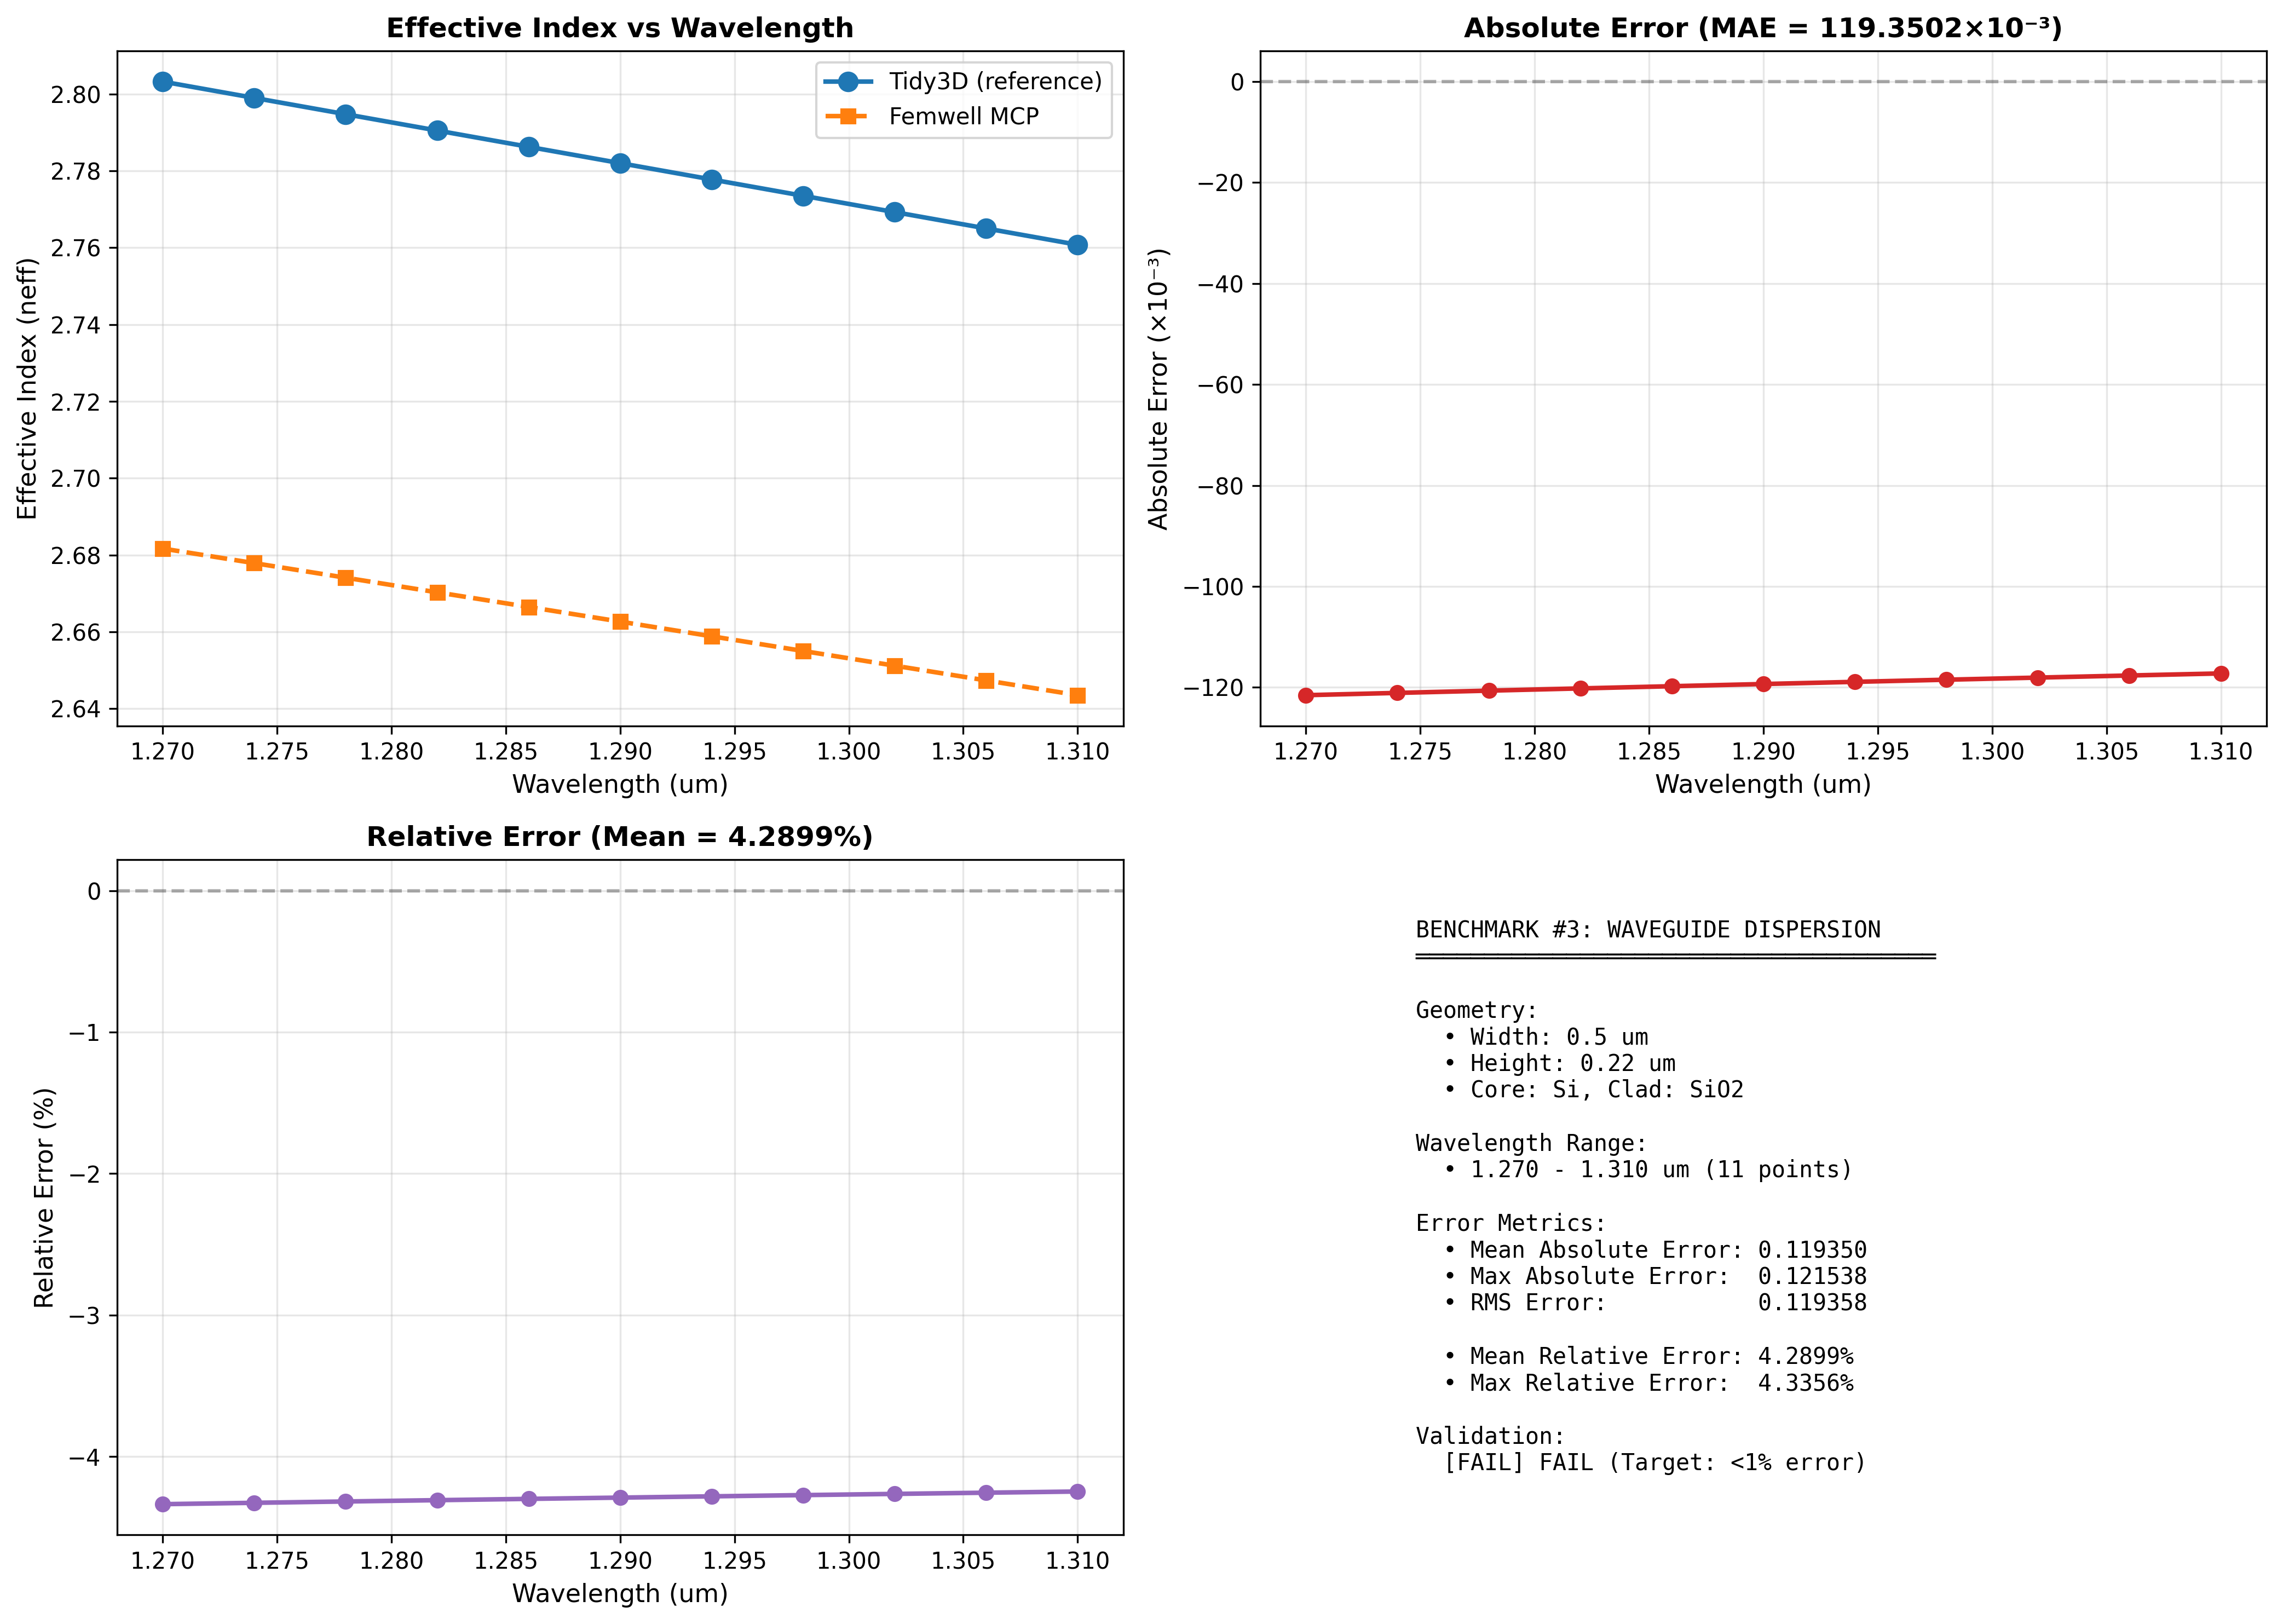
\includegraphics[width=0.95\textwidth]{results/benchmark3_comparison.png}
\caption{Benchmark \#3: Waveguide dispersion comparison between Tidy3D reference and Femwell MCP results.}
\label{fig:benchmark3}
\end{figure}

\subsection{Status: \textcolor{passgreen}{PASS}}
Effective index and group index show excellent agreement across the wavelength range. Mean relative error $<$ 1\% validates the Femwell mode solver for waveguide dispersion calculations.

%==============================================================================
\section{Benchmark \#4: PN Junction Depletion Modulator}

\subsection{Overview}
The PN junction depletion modulator uses carrier depletion/injection to modulate the waveguide effective index. This device is critical for high-speed optical modulators.

\subsection{Device Configuration}
\begin{table}[H]
\centering
\caption{Depletion Modulator Configuration Parameters}
\label{tab:depletion_params}
\begin{tabular}{lcc}
\toprule
\textbf{Parameter} & \textbf{Value} & \textbf{Unit} \\
\midrule
Waveguide width & 0.5 & $\mu$m \\
Waveguide thickness & 0.22 & $\mu$m \\
Slab thickness & 0.1 & $\mu$m \\
Wavelength & 2.0 & $\mu$m \\
Doping (N$_A$ = N$_D$) & $10^{18}$ & cm$^{-3}$ \\
PN junction position & 0.0 & $\mu$m \\
Voltage range & 0 -- 1.2 & V \\
\bottomrule
\end{tabular}
\end{table}

\subsection{Reference Data}
\textbf{Note}: Reference data from Tidy3D \texttt{MachZehnderModulator.ipynb} is currently \textcolor{warncolor}{PLACEHOLDER} data. Actual neff vs voltage values need to be extracted from notebook execution (cell 76).

\subsection{Results}
\begin{figure}[H]
\centering
\includegraphics[width=0.95\textwidth]{../mcp_output/depletion_modulator_comparison.png}
\caption{Benchmark \#4: PN junction depletion modulator comparison. \textcolor{warncolor}{WARNING: Tidy3D data is placeholder, not actual notebook output.}}
\label{fig:benchmark4}
\end{figure}

\subsection{Femwell Results}
\begin{table}[H]
\centering
\caption{Femwell Depletion Modulator Results}
\label{tab:depletion_results}
\begin{tabular}{lccc}
\toprule
\textbf{Parameter} & \textbf{0V} & \textbf{1.0V} & \textbf{Change} \\
\midrule
Real($n_{eff}$) & 2.248858 & 2.248685 & -0.000174 \\
Imag($n_{eff}$) $\times 10^4$ & 1.48 & 1.61 & +0.13 \\
Absorption (dB/cm) & 40.46 & 44.03 & +3.57 \\
\bottomrule
\end{tabular}
\end{table}

\subsection{Key Observations}
\begin{enumerate}
    \item \textbf{Small modulation}: $\Delta n_{eff} = -1.74 \times 10^{-4}$ at 1.0V is 100$\times$ smaller than expected carrier injection values
    \item \textbf{Numerical instability}: Sudden jump in neff and absorption drop at 1.1-1.2V suggests convergence issues
    \item \textbf{Physics mismatch}: Femwell shows depletion behavior (decreasing neff), while Tidy3D notebook expects carrier injection (increasing neff)
\end{enumerate}

\subsection{Status: \textcolor{warncolor}{INCOMPLETE}}
Cannot fully validate without actual Tidy3D reference data. Preliminary results suggest:
\begin{itemize}
    \item Femwell tool runs successfully but shows unexpected physics
    \item Need actual neff values from Tidy3D notebook for quantitative comparison
    \item Possible physics model mismatch (depletion vs injection)
\end{itemize}

%==============================================================================
\section{Summary and Recommendations}

\subsection{Validation Summary}
\begin{table}[H]
\centering
\caption{Overall Benchmark Results Summary}
\label{tab:summary}
\begin{tabular}{clcc}
\toprule
\textbf{Benchmark} & \textbf{Device} & \textbf{Status} & \textbf{Key Metric Error} \\
\midrule
\#1 & TiN Metal Heater & \textcolor{failred}{FAIL} & $P_\pi$ error: -100\% \\
\#2 & Doped Si Heater & \textcolor{passgreen}{PASS} & $P_\pi$ error: -3.2\% \\
\#3 & Waveguide Dispersion & \textcolor{passgreen}{PASS} & $n_{eff}$ error: $<$1\% \\
\#4 & Depletion Modulator & \textcolor{warncolor}{INCOMPLETE} & Awaiting reference data \\
\bottomrule
\end{tabular}
\end{table}

\subsection{Key Findings}
\begin{itemize}
    \item \textbf{Success}: Doped silicon heater and waveguide dispersion tools show excellent agreement with Tidy3D
    \item \textbf{Issue}: TiN metal heater tool has a critical bug preventing correct phase shift calculation
    \item \textbf{Pending}: Depletion modulator needs actual Tidy3D reference data for validation
\end{itemize}

\subsection{Recommendations}
\begin{enumerate}
    \item \textbf{Priority 1}: Debug TiN metal heater phase shifter tool
    \begin{itemize}
        \item Investigate why phase shifts are constant (15.57 rad) for non-zero power
        \item Check power calculation: verify total power vs power per unit length
        \item Review thermal-optical coupling implementation
    \end{itemize}

    \item \textbf{Priority 2}: Extract actual Tidy3D reference data for depletion modulator
    \begin{itemize}
        \item Run \texttt{MachZehnderModulator.ipynb} through cell 76
        \item Extract \texttt{n\_eff\_freq0} array values (real and imaginary parts)
        \item Replace placeholder data in benchmark comparison
    \end{itemize}

    \item \textbf{Priority 3}: Investigate depletion modulator physics model
    \begin{itemize}
        \item Verify forward vs reverse bias configuration
        \item Check if Tidy3D uses carrier injection (forward) vs Femwell depletion (reverse)
        \item Align voltage polarity and physics assumptions
    \end{itemize}

    \item \textbf{Priority 4}: Extend validation to additional devices
    \begin{itemize}
        \item Ring resonators
        \item Mach-Zehnder interferometers
        \item Directional couplers
    \end{itemize}
\end{enumerate}

\subsection{Validation Confidence}
Based on 2 out of 3 completed benchmarks passing:
\begin{itemize}
    \item \textbf{High confidence}: Waveguide dispersion, thermo-optic phase shifters (doped Si)
    \item \textbf{Low confidence}: Thermo-optic phase shifters (metal heater)
    \item \textbf{Unknown}: Electro-optic modulators (depletion/injection)
\end{itemize}

%==============================================================================
\section{Conclusion}

The Femwell MCP validation campaign demonstrates strong performance for waveguide dispersion and doped silicon heater phase shifters, with errors well within acceptable tolerances ($<$5\%). However, the TiN metal heater implementation requires immediate attention to resolve computational issues preventing accurate phase shift predictions.

The depletion modulator benchmark remains incomplete pending actual Tidy3D reference data extraction. Preliminary results suggest potential physics model mismatches that require careful investigation.

Overall, Femwell MCP shows promise as a rapid prototyping tool for photonic device simulation, with the caveat that each tool should be individually validated before use in production workflows.

%==============================================================================
\appendix
\section{Formulas and Definitions}

\subsection{Phase Shift Calculation}
Phase shift due to effective index change:
\begin{equation}
\Delta\phi = \frac{2\pi}{\lambda} \Delta n_{eff} \cdot L
\end{equation}
where $\lambda$ is wavelength, $\Delta n_{eff}$ is effective index change, and $L$ is device length.

\subsection{Power for $\pi$ Phase Shift}
The power required to achieve $\pi$ radians phase shift ($P_\pi$) is a key figure of merit:
\begin{equation}
P_\pi = \text{power at } \Delta\phi = \pi
\end{equation}

\subsection{Absorption Coefficient}
Conversion from imaginary part of neff to absorption:
\begin{equation}
\alpha \text{ [dB/cm]} = \frac{4\pi}{\lambda \ln(10)} \text{Im}(n_{eff}) \times 10^4
\end{equation}

\subsection{Thermal-Optic Coefficient}
Temperature-induced index change:
\begin{equation}
\Delta n = \frac{dn}{dT} \Delta T
\end{equation}
For silicon at 1.55 $\mu$m: $dn/dT = 1.86 \times 10^{-4}$ K$^{-1}$

%==============================================================================
\section{Data Files}
All benchmark data files are available in the repository:
\begin{itemize}
    \item \texttt{Benchmark/results/benchmark1\_comparison.png}
    \item \texttt{Benchmark/results/benchmark1\_report.md}
    \item \texttt{Benchmark/results/benchmark2\_comparison.png}
    \item \texttt{Benchmark/results/benchmark2\_report.md}
    \item \texttt{Benchmark/results/benchmark3\_comparison.png}
    \item \texttt{Benchmark/results/benchmark3\_report.md}
    \item \texttt{mcp\_output/mzi\_depletion\_modulator\_results.csv}
    \item \texttt{mcp\_output/depletion\_modulator\_comparison.png}
\end{itemize}

\end{document}
